\section{The linear case}
	When travelling through space with acceleration, there are two possible basic paths that the travelling ship
	can take. One is a linear shape as shown below.
	\begin{figure}[H]
	\caption{Diagram of the spaceship taking a linear path.}
	\label{fig:linearCase}
	\centering
	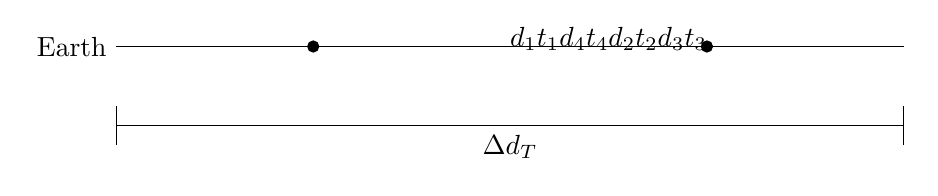
\begin{tikzpicture}
		\coordinate [label=left:Earth] (E) at (-5,0);
		\coordinate (N) at (5,0);
		\coordinate (M) at (0,0);
		\coordinate (Me) at (-2.5,0);
		\coordinate (Mn) at (2.5,0);

		\coordinate (TL) at (-5,-1);
		\coordinate (TR) at (5,-1);
		\coordinate [label=below:$\Delta d_T$](T) at (0,-1);

		\draw (E) -- (N);
		\draw (TL) -- (TR);
		\draw (-5,-0.75) -- (-5,-1.25);
		\draw (5,-0.75) -- (5,-1.25);

		\tkzLabelSegment[above=1em](E,Me){$\Del d_1$};
		\tkzLabelSegment[above](E,Me){$\Del t_1$};
		\tkzLabelSegment[above=1em](Me,M){$\Del d_4$};
		\tkzLabelSegment[above](Me,M){$\Del t_4$};

		\tkzLabelSegment[above=1em](M,Mn){$\Del d_2$};
		\tkzLabelSegment[above](M,Mn){$\Del t_2$};
		\tkzLabelSegment[above=1em](Mn,N){$\Del d_3$};
		\tkzLabelSegment[above](Mn,N){$\Del t_3$};

		\filldraw[black] (E) circle (2pt);
		\filldraw[black] (N) circle (2pt);
		\filldraw[black] (M) circle (2pt);
	\end{tikzpicture}
\end{figure}

	In this path, the ship will accelerate forward (away from the earth) in a straight line for a time $\Del t_1$, then it will begin 
	to decelerate at the same rate opposite to it's velocity for a time $\Del t_2$ until it reaches a halt. The ship will then 
	accelerate backwards (towards the earth) in a straight line for a time $\Del t_3$, and finally, it will decelerate for a time
	$\Del t_4$ until it reaches a halt at it's starting position (position of the earth).

	Given that the acceleration of the ship is constant, it is sufficient to say that $\Del t_1 = \Del t_2$ since the 
	ship must decelerate at the same rate at which it accelerates. Given this, it is also sufficient to say that $\Del t_3 = \Del t_4$.
	We can also say that $\Del d_1 + \Del d_2 = \Del d_3 + \Del d_4$ given that the distance travelled to and from the turning point
	must be equal. This means that $\Del t_1 + \Del t_2 = \Del t_3 + \Del t_4$ meaning: $Del t_1 = \Del t_2 = \Del t_3 = \Del t_4$.

	Since the acceleration and deceleration times are all equal: $\Del T_T = 4\Del t_1$.

	Since the simulator will calculate the values using a summation technique, the time dilation over an accelerating time frame will be 
	equal to the time dilation over an equal time frame decelerating with the same acceleration magnitude. This means that the time dilation
	over the time frame $\Del t_1$ is equal to the dilation over the other three time frames, thus the simulator will only calculate
	the dilation for the first time frame, and will multiply the result by 4 for the final dilation.
	\begin{samepagecols}{2}
		\[\Del d_1 + \Del d_2 + \Del d_3 + \Del d_4 = \Del d_T\]
		\[\Del d_1 = \Del d_2 = \Del d_3 = \Del d_4\]
		\[\Del d_T = 4\Del d_1\]

		\columnbreak

		\[\Del t_1 + \Del t_2 + \Del t_3 + \Del t_4 = \Del t_T\]
		\[\Del t_1 = \Del t_2 = \Del t_3 = \Del t_4\]
		\[\Del t_T = 4\Del t_1\]
	\end{samepagecols}
